% Copyright 2004 by Till Tantau <tantau@users.sourceforge.net>.
%
% In principle, this file can be redistributed and/or modified under
% the terms of the GNU Public License, version 2.
%
% However, this file is supposed to be a template to be modified
% for your own needs. For this reason, if you use this file as a
% template and not specifically distribute it as part of a another
% package/program, I grant the extra permission to freely copy and
% modify this file as you see fit and even to delete this copyright
% notice.

\documentclass{beamer}

\usetheme{classic}

\usefonttheme{professionalfonts} % using non standard fonts for beamer
\usefonttheme{serif} % default family is serif
\usepackage{fontspec} % Allows font customization
\defaultfontfeatures{Mapping=tex-text,Scale=MatchLowercase}
\setmainfont{Ubuntu Light} % Main document font

\usepackage{hyperref}
\usepackage[english,spanish]{babel}

\usepackage{minted}

\usemintedstyle{friendly}

\newminted{java}{
fontsize=\small,
   gobble=4,
   frame=lines,
   framesep=2mm,
   mathescape=true,
}
\newminted{xml}{
fontsize=\small,
   gobble=0,
   frame=lines,
   framesep=2mm,
   mathescape=true,
}

\title{Curso de programación Android}

% A subtitle is optional and this may be deleted
\subtitle{T-Formación}

\author{Alejandro~Alcalde}
% - Give the names in the same order as the appear in the paper.
% - Use the \inst{?} command only if the authors have different
%   affiliation.

\institute[Estudiante de la ETSIIT] % (optional, but mostly needed)
{
  \href{http://elbauldelprogramador.com}{elbauldelprogramador.com}}
% - Use the \inst command only if there are several affiliations.
% - Keep it simple, no one is interested in your street address.

\date{\today}
% - Either use conference name or its abbreviation.
% - Not really informative to the audience, more for people (including
%   yourself) who are reading the slides online

\subject{Curso Programación Android}
% This is only inserted into the PDF information catalog. Can be left
% out.

% If you have a file called "university-logo-filename.xxx", where xxx
% is a graphic format that can be processed by latex or pdflatex,
% resp., then you can add a logo as follows:

%\pgfdeclareimage[height=0.1cm]{university-logo}{university-logo-filename}
%\logo{\pgfuseimage{university-logo}}
%\titlegraphic{
\includegraphics{university-logo-filename}}

% Delete this, if you do not want the table of contents to pop up at
% the beginning of each subsection:
\AtBeginSubsection[]
{
  \begin{frame}<beamer>{Contenidos}
    \tableofcontents[currentsection,currentsubsection]
  \end{frame}
}

% Let's get started
\begin{document}

\begin{frame}
  \titlepage
\end{frame}

\begin{frame}{Contenidos}
  \tableofcontents
  % You might wish to add the option [pausesections]
\end{frame}

\section{Conceptos básicos Android}

% You can reveal the parts of a slide one at a time
% with the \pause command:
\begin{frame}{Conceptos básicos Android}
  \begin{itemize}
    \item {\textbf{View:} Representa el componente básico en el que se apoyan todos los elementos que construyen una interfaz. Todos los elementos que generan interfaces heredan de la clase \texttt{\href{http://developer.android.com/reference/android/view/View.html}{View}}
    \pause
    }

  \item<2-> {
    \textbf{Activity:} Encargada de mostrar la interfaz de usuario e interactuar con él. Responden a los eventos generados por el usuario (pulsar botones etc). Heredan de la clase \href{http://developer.android.com/reference/android/app/Activity.html}{\texttt{Activity}}.
  }
  \item<3-> { \textbf{Services:} No tienen interfaz visual y se ejecutan en segundo plano, se encargan de realizar tareas que deben continuar ejecutandose cuando nuestra aplicación no está en primer plano. Todos los servicios extienden de la clase \texttt{\href{http://developer.android.com/reference/android/app/Service.html}{Service}}
  }
  \end{itemize}
\end{frame}

\begin{frame}{Conceptos básicos Android}
  \begin{itemize}
  \item{
    \textbf{Content Provider:} Ponen un grupo de datos a disposición de distintas aplicaciones, extienden de la clase ContentProvider para implementar los métodos de la interfaz, pero para acceder a esta interfaz se ha de usar una clase llamada ContentResolver.
    \pause
  }
  \item<2-> {
    \textbf{BroadcastReceiver:} Simplemente reciben un mensaje y reaccionan ante él, extienden de la clase BroadcastReceiver, no tienen interfaz de usuario, pero pueden lanzar Actividades como respuesta a un evento o usar NotificationManager para informar al usuario.
  }
  % or you can use the \uncover command to reveal general
  % content (not just \items):
  \item<3-> {
    \textbf{Intent:} Permite realizar la comunicación y transferencia de datos entre objetos de la clase Activity o Service. También permite iniciar otras Activities o lanzar otras aplicaciones.
  }
  \end{itemize}
\end{frame}

\section{Hola Mundo}

\subsection{Crear el proyecto}

\begin{frame}{Crear el proyecto}
\begin{block}{Pasos a realizar}
En Android Studio, File » New Project.
\end{block}
\end{frame}

\subsection{Componentes del proyecto}

\begin{frame}{Componentes del proyecto}
\begin{block}{}
Los proyectos de Android siguen una estructura fija de carpetas que debemos respetar.
\begin{figure}[H]
\centering
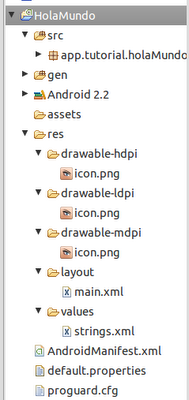
\includegraphics[scale=.3]{./img/estructuraCarpetas.png}
\end{figure}
\end{block}
\end{frame}

\subsubsection{Carpeta Res}

\begin{frame}{Carpeta Res}
\begin{block}{}
Ésta es una de las carpeta que más se va a usar junto con \texttt{src}. Se compila y se generan referencias en la clase \texttt{R}, para acceder a ellos desde código. Están escritos en \texttt{XML}.
\pause
\end{block}
\begin{itemize}
    \item<2-> \texttt{anim}: Definición de Animaciones.
    \item<3-> \texttt{color}: Definición de colores
    \item<4-> \texttt{drawable}: Ficheros bitmap(.png, .9.png, .jpg, .gif) o XML con contenidos que se dibujarán (fondos, botones etc).
    \item<5-> \texttt{layout}: Definen la capa de interfaz de usuario
    \item<6-> \texttt{menu}: Definición de los menús de la aplicación
    \item<7-> \texttt{raw}: Binarios que no se pueden colocar en las otras carpetas.
    \item<8-> \texttt{values}: Definición de estilos, cadenas de texto para Localización etc.
    \item<9-> \texttt{xml}: Ficheros XML que pueden ser accedidos en tiempo de ejecución
\end{itemize}
\end{frame}

\begin{frame}[fragile]{Hola Mundo}
\begin{block}{}
\begin{javacode}
    @Override
    protected void onCreate(Bundle savedInstanceState) {
        super.onCreate(savedInstanceState);

        /**
         * Método encargado de “inflar” la actividad.
         * Inicializar cada componente de la actividad
         * con su correspondiente View.
         */
        setContentView(R.layout.activity_main);
    }
\end{javacode}
\end{block}
\end{frame}

\begin{frame}{Ciclo de vida de una Activity}
\begin{block}{}
\begin{figure}[H]
\centering
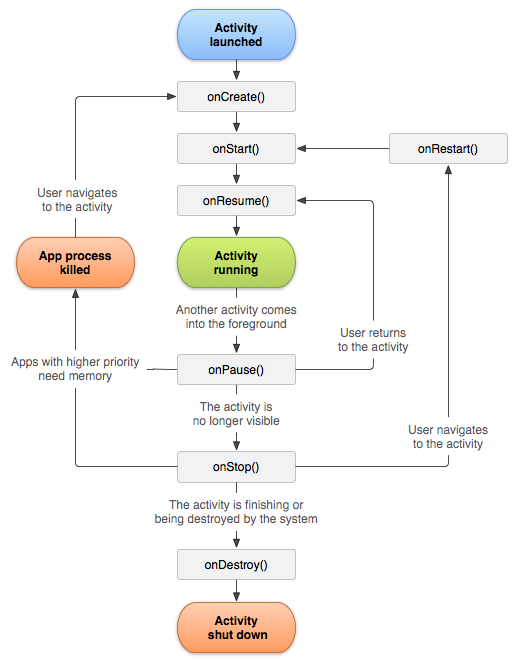
\includegraphics[scale=.33]{./img/activityLifecycle.png}
\end{figure}
\end{block}
\end{frame}

\begin{frame}[fragile]{Hola Mundo}
\begin{block}{}
\textbf{./res/layout/activity\_main.xml}
\begin{xmlcode}
<RelativeLayout
    android:layout_width="match_parent"
    android:layout_height="match_parent"
    tools:context=".MainActivity" >
    <TextView
        android:layout_width="wrap_content"
        android:layout_height="wrap_content"
        android:text="@string/hello_world" />
</RelativeLayout>
\end{xmlcode}
\textbf{./res/values/strings.xml}
\begin{xmlcode}
<resources>
    <string name="hello_world">Hello world!</string>
</resources>
\end{xmlcode}
\end{block}
\end{frame}
% Placing a * after \section means it will not show in the
% outline or table of contents.
\section*{Qué hemos visto}

\begin{frame}{Qué hemos visto}
  \begin{itemize}
  \item
    Cómo preparar el entorno para desarrollar aplicaciones Android.
  \item
    Conceptos básicos Android.
  \item
    Creación de un proyecto Hola Mundo.
  \end{itemize}
\end{frame}

\begin{frame}{¿Y ahora qué?}
  \begin{itemize}
  \item
    A partir de ahora, trabajaremos sobre ejemplos funcionales, deteniéndonos en las partes de código importantes para explicarlas.
  \end{itemize}
\end{frame}

\section{Interfaz gráfica}
\subsection{Conceptos básicos}
\begin{frame}{Conceptos básicos Android}
    \begin{block}{}Todos los componentes de la interfaz de usuario de Android descienden de la clase \textit{View}. Dichos objetos están organizados en forma de árbol y pueden contener nuevos objetos View, permitiendo crear interfaces muy completas.

Los objetos \textit{{View}}\index{View} se pueden definir de dos maneras:
\begin{itemize}
    \item {
        Mediante un fichero XML colocado dentro del directorio \textit{{res/layout}}, que es el que usaremos normalmente.\pause
    }
    \item <2->{
        En tiempo de ejecución, muy útil para crear nuestros propios componentes View.
    }
\end{itemize}
Para dibujar la interfaz, el sistema necesita que le pasemos el objeto View raiz, para ir descendiendo por cada uno de sus nodos y presentar al usuario toda la interfaz. El método encargado de esto es \textit{{Activity.setContentView()}}.\index{setContentView()}
    \end{block}
\end{frame}

\begin{frame}{Conceptos básicos Android}
    \begin{block}{}
Para que Android sepa dibujar correctamente los objetos, tenemos que pasarle algunos datos, como son la altura y anchura. Para eso nos servimos de la clase \textit{{LayoutParams}}\index{LayoutParams}, que puede tomar los siguientes valores:
    \begin{itemize}
    \item Un número. \pause
    \item <2-> La constante \textit{MATCH\_PARENT}\index{MATCH\_PARENT}, que indica que la vista debe intentar ser tan grande como su padre, quitando el padding.
    \item <3-> La constante \textit{WRAP\_CONTENT}\index{WRAP\_CONTENT}, para que intente ser lo suficientemente grande para mostrar su contenido, mas el padding.
    \end{itemize}
    \end{block}
\end{frame}

\begin{frame}{Conceptos básicos Android}
    \begin{block}{}
    Un atributo imprescindible es el \textit{{id}}(de tipo entero). Que sirve para identificar únicamente a un objeto View. Cuando lo declaramos mediante xml podemos referenciarlo a través de la clase de recursos R, usando una @.

    Los objetos View pueden tener otros muchos atributos, como padding, colores, imágenes, fondos, márgentes etc.
        \begin{itemize}
                \item \textit{\textbf{android:id=“@+id/nombreID”:}}
                Crea un nuevo atributo en la clase R llamado nombreID.\pause
                \item <2-> \textit{\textbf{android:id=“@id/nombreID”:}}
                Hace referencia a un id ya existente asociado a la etiqueta 'nombreID'.
                \item <3-> \textit{\textbf{android:id=“@android:id/list”:}}
                Referencia a un a etiqueta definida en la clase R del sistema llamada 'list'.
        \end{itemize}
    \end{block}
\end{frame}

\section{Layouts}

\begin{frame}{Qué es un layout}
    \begin{block}{}
Los layout\index{layout} nos permiten posicionar cada objeto gráfico en el lugar que queramos de la pantalla, es decir, nos permite diseñar el aspecto gráfico que va a tener nuestra pantalla. Los layouts son de tipo ViewGroup\index{ViewGroup}, una subclase de View\index{View}.

Existen varios tipos de Layouts para Android, vamos a ver los más comunes:
    \end{block}
\end{frame}

\subsection{LinearLayout}
\begin{frame}{LinearLayout}
    \begin{block}{}
    Este tipo de layout coloca sus hijos unos detrás de otros, comenzando por la esquina superior izquierda de la pantalla. Podemos colocarlos alineados horizontalmente o verticalmente mediante su propiedad \textit{{android:orientation=“horizontal | vertical”}}.
\begin{figure}[h]
    \centering
\includegraphics[scale=.35]{./img/LinearLayout.png}
    \caption{LinearLayout}
\end{figure}
\end{block}
\end{frame}

\begin{frame}[fragile]{LinearLayout}
    \begin{block}{}
\begin{xmlcode}
<linearlayout
    android:orientation="horizontal"
    android:layout_width="match_parent"
    android:layout_height="match_parent">

    <textview android:layout_width="wrap_content"
        android:layout_height="wrap_content"
        android:text="@string/app_name"
        android:background="#0ff"/>

    <textview android:layout_width="wrap_content"
        android:layout_height="wrap_content"
        android:text="@string/hello"
        android:background="#ff0"/>
</linearlayout>
\end{xmlcode}
    \end{block}
\end{frame}

\subsection{RelativeLayout}

\begin{frame}{RelativeLayout}
    \begin{block}{}
Este Layout permite que coloquemos los elementos en un lugar con respecto a la posición de otro, es decir, colocar un botón a la derecha de un texto, o centrarlo en la pantalla, o por ejemplo, colocar un texto encima de tal elemento y a la derecha de este otro.

Para conseguir esto, \textit{{RelativeLayout}} proporciona propiedades como \textit{{android:layout\_toRightOf}} o \textit{{android:layout\_alignLeft}}, que toman como valores los identificadores de los objetos, o valores booleanos.
    \end{block}
\end{frame}

\begin{frame}
    \begin{block}{}
\begin{figure}[H]
    \centering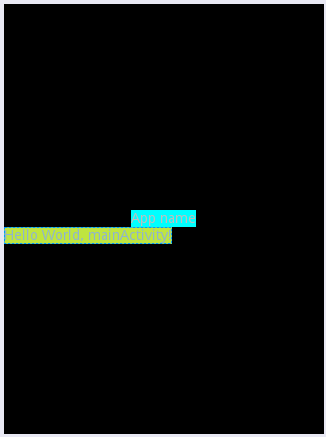
\includegraphics[scale=.45]{./img/RelativeLayout.png}
    \caption{RelativeLayout}
\end{figure}
    \end{block}
\end{frame}

\begin{frame}[fragile]{RelativeLayout}
    \begin{block}{}
\begin{xmlcode}
<relativelayout
    android:orientation="horizontal"
    android:layout_width="match_parent"
    android:layout_height="match_parent">
    <textview android:layout_width="wrap_content"
        android:layout_height="wrap_content"
        android:text="@string/app_name"
        android:background="#0ff"
        android:layout_centerInParent="true"
        android:id="@+id/text1"/>
    <textview android:id="@+id/text2"
        android:layout_width="wrap_content"
        android:layout_height="wrap_content"
        android:text="@string/hello"
        android:background="#ff0"
        android:layout_below="@id/text1"/>
</relativelayout>
\end{xmlcode}
    \end{block}
\end{frame}

\subsection{Notificaciones y Diálogos}
\begin{frame}{Notificaciones y Diálogos}
    \begin{block}{}En ocasiones hay que mostrar mensajes al usuario para
    informarle del estado de la aplicación, o del estado de las operaciones 
    que se estén llevando a cabo. Hay 3 tipos:

	\begin{itemize}
		\item {
			Notificaciones Toast.\pause
		}
		\item {
			Notificaciones en la barra de estado.
		}
		\item <3->{
			Diálogos.
		}
	\end{itemize}
Para dibujar la interfaz, el sistema necesita que le pasemos el objeto View raiz, para ir descendiendo por cada uno de sus nodos y presentar al usuario toda la interfaz. El método encargado de esto es \textit{{Activity.setContentView()}}.\index{setContentView()}
    \end{block}
\end{frame}

\section{Fragments}
\begin{frame}{Fragments}
    \begin{itemize}
        \item {
            Permiten encapsular componentes de la interfaz para reutilizarlos. \pause
        }
        \item <2->{
            Clase Fragment, puede definir su propio layout y maneja su ciclo de vida.
        }
        \item <3->{
            Se puede configurar junto con otros fragments dentro de una actividad para adaptarlo al tamaño de la pantalla.
        }
    \end{itemize}
\end{frame}

\section{Persistencia de datos}
\begin{frame}{Persistencia de datos}
    \begin{block}{}
        La mayoría de apps necesitan guardar datos, ya sea para no perder la información cuando se ejecuta
        el método onPause(), información de preferencias  o cantidades mayores de información en bases de datos.
        Los distintos métodos de almacenamiento disponibles son:
    \end{block}
    \begin{itemize}
        \pause
        \item {
            Pares clave-valor de tipos de datos simples en un fichero Shared Preference.\pause
        }
        \item <2->{
            Ficheros de cualquier tipo en el sistema de archivos.\pause
        }
        \item <3->{
            Bases de datos en SQLite.
        }
    \end{itemize}
\end{frame}

\section{Interactuar con otras aplicaciones}
\begin{frame}{Interactuar con otras aplicaciones}
    \begin{block}{}
        Ya hemos visto cómo usar Intents para comunicar actividades de la misma app. Cuando un intent se lanza
        al sistema en lugar de a otra activiy, se usa para iniciar el componente apropiado de una aplicación.\\
        Hay dos tipos de Intents:
    \end{block}
    \begin{itemize}
        \pause
        \item {
            \emph{Explícito:} Para iniciar un componente específico (Un activity concreto).\pause
        }
        \item<1->{
            \emph{Implícito:} Para iniciar cualquier componente que pueda controlar la acción requerida. (Echar una foto).
        }
    \end{itemize}
\end{frame}

\section{Interactuar con otras aplicaciones}
\begin{frame}{Interactuar con otras aplicaciones}
    \begin{block}{}
        Con los intents se puede:
    \end{block}
    \begin{itemize}
        \item {
            Mover de una pantalla a otra dentro de nuestra app.\pause
        }
        \item {
            Mandar al usuario a la pantalla de otra aplicación para realizar una acción.
        }
        \item<3->{
            Cualquier pantalla a la que invoquemos puede devolver un resultado.
        }
        \item<4->{
            Podemos permitir que otras aplicaciones lancen una actividad de la nuestra.
        }
    \end{itemize}
\end{frame}

\section{Componentes Gráficos y eventos}
\begin{frame}{Componentes Gráficos y eventos}
    \begin{block}{}
        Para que una aplicación sea funcional debe responder a los eventos
        del usuario. Los más típicos son:
    \end{block}
    \begin{itemize}
        \item {
            \textit{onClickListener:} Para botones, texto, en general, para todos los Views.\pause
        }
        \item {
            \textit{onKeyListener:} Para cajas de texto.
        }
        \item<3->{
            \textit{onCheckedChangeListener:} Para checkboxes.
        }
        \item<4->{
            \textit{onItemClickListener:} Elementos de un ListView
        }
    \end{itemize}
\end{frame}

\section{Menús}
\begin{frame}{Menús}
    \begin{block}{}
        Veremos cómo crear menús con Action Bar, ya que los menús estándar
        están anticuados. Los tres tipos fundamentales de menús son:
    \end{block}
    \begin{itemize}
        \item {
            \textbf{Options menu y action bar:} Elementos principales del menú.
            Aquí deben ir acciones que tienen un impacto global en la app. (buscar, ajustes, crear mensaje etc)\pause
        }
        \item {
            \textbf{Context menu y contextual action mode:} Menús basados
            en el contexto. Son menús flotantes que aparecen al realizar un “long-click”
            en algún elemento. Las acciones se realizan sobre el contenido
            seleccionado. (Ej. Al seleccionar texto, copiar, pegar...)
        }
    \end{itemize}
\end{frame}

\section{Adaptadores}
\begin{frame}{Adaptadores}
    \begin{itemize}
        \item {
            Puete entre un AdapterView y los datos de una Vista (View)\pause
        }
        \item {
           Colecciones de datos que asignamos a una vista para que ésta los muestre. (Un ListView p.e)
        }
    \end{itemize}
\end{frame}


% All of the following is optional and typically not needed.
\appendix
\section<presentation>*{\appendixname}
\subsection<presentation>*{Bibliografía recomendada}

\begin{frame}[allowframebreaks]
  \frametitle<presentation>{Bibliografía recomendada}

  \begin{thebibliography}{10}

  \beamertemplatebookbibitems

  \bibitem{ProAnd4}
    Satya~Komatineni.
    \newblock {\em \href{http://www.amazon.es/gp/product/1430239301/ref=as_li_ss_tl?ie=UTF8&camp=3626&creative=24822&creativeASIN=1430239301&linkCode=as2&tag=elbaudelpro-21}{Pro Android 4 - Libro en Amazon}}.
    \newblock Apress 2012.


  \beamertemplatearticlebibitems
  % Followed by interesting articles. Keep the list short.

  \bibitem{developerandroid}
    Developer.android.com
    \newblock Documentación oficial de Android.
    \newblock {\em \href{http://developer.android.com/develop/index.html}{developer.android.com}}
  \end{thebibliography}
\end{frame}

\end{document}


